\chapter{Implementation}
\label{cha:implementation}

This chapter will describe in detail the technical implementation of the Omni platform.

\section{Configuration}
Configuration is an important part of any production application. It is any data required by the application for it to run.
Configuration may need to change, and it should be able to do so without requiring developers to rebuild the application.
Allowing configuration to be ephemeral enables companies with separate teams that manage a platform's operations to make configuration changes without the need for intervention by a software developer.

Configuration items should be passed to the application via its environment rather than compiled into its binary.
One method for specifying configuration is through a configuration file. This file (normally JSON or YAML) contains key-value pairs of data for the application to consume at start-up.
Some frameworks even enable the file to be monitored for changes so that the most up-to-date values can be used without requiring a restart. 

Another method preferred in Kubernetes and containerised environments is using environment variables.
These are variables set in the bash environment that the application is executed from. The application can then read the values of these variables and use them for its own configuration.

Kubernetes allows environment variables to be specified in the workload manifests for each application.
This means that if the configuration changes, a new manifest can be loaded to bring new pods online with the updated config. Once the new pods are available and responding to requests, the old pods can be scaled down and removed.

\lstinputlisting[language=Go, caption=Example of Parsing Environment Variables, label={lst:go-env}]{code-snippets/go-env-example.go.bak}

The second method will be used as Omni is designed for Kubernetes. To enable the use of environment variables for configuration, an open-source package called \underline{\href{https://github.com/caarlos0/env}{Caarlos0/env}} \nocite{env} will automatically pull these values from the environment (shown in Listing \ref{lst:go-env}).
Defined in the applications are different configuration objects with the required configuration items included, along with some special tags that indicate the name of the related environment variable.
On start-up, a call to the package automatically creates the configuration objects based on the values from the environment. The config objects can then be passed around the application to the sections of code that require them.

\section{Observability}
Logging and observability are vital to the ongoing stability of any production system. ``The distributed nature of microservices also introduces complexity, making  it  challenging  to  ensure  the  reliability,  performance,  and  security  of  the  system'' \citep{chinamanagonda2022observability}.
Clear and consistent logs are crucial for developers to be able to debug faulty platforms quickly. 

Logging is not the only facet of observability. However, metrics and tracing are also key to building a holistic view of a platform's health.
Metrics are the key numerical data points representing a system's health and behaviour over time.
Metrics often include requests per second, latency and CPU usage. These can be easily aggregated, structured, and visualised in top-level dashboards to provide a glanceable overview of how a platform is performing.
They are the first level of reporting an operations team will monitor.

Traces, on the other hand, record the path that requests take through a platform. They often capture the logs each system produces along the way and measure latencies across the system.
Traces are ideal for identifying bottlenecks and pinpointing failures within a larger microservices architecture. Tracing is often handled by a framework called \underline{\href{https://opentelemetry.io}{Open Telemetry}} \nocite{opentel}, a standardised way of collecting and exporting traces from many different applications.

Finally, logs are the lowest level of the three fundamental observability pillars. Logs are immutable, and applications emit timestamped events to process incoming requests.
Developers with a fine-grained understanding of how the system functions best use logs, which are extremely useful for pinpointing the exact line where a system has failed. 

\subsection{Observability in Omni}
In Omni, the Go standard library's structured logger emits logs, allowing each log to contain extra information, such as variables.
The structured logger can output logs in various formats, the most common being text-based (for console logs) and JSON-based (for consumption into an observability pipeline).

\lstinputlisting[language=Go, caption=Example of Structured Logging]{code-snippets/go-logger-example.go.bak}

\begin{figure}[htbp]
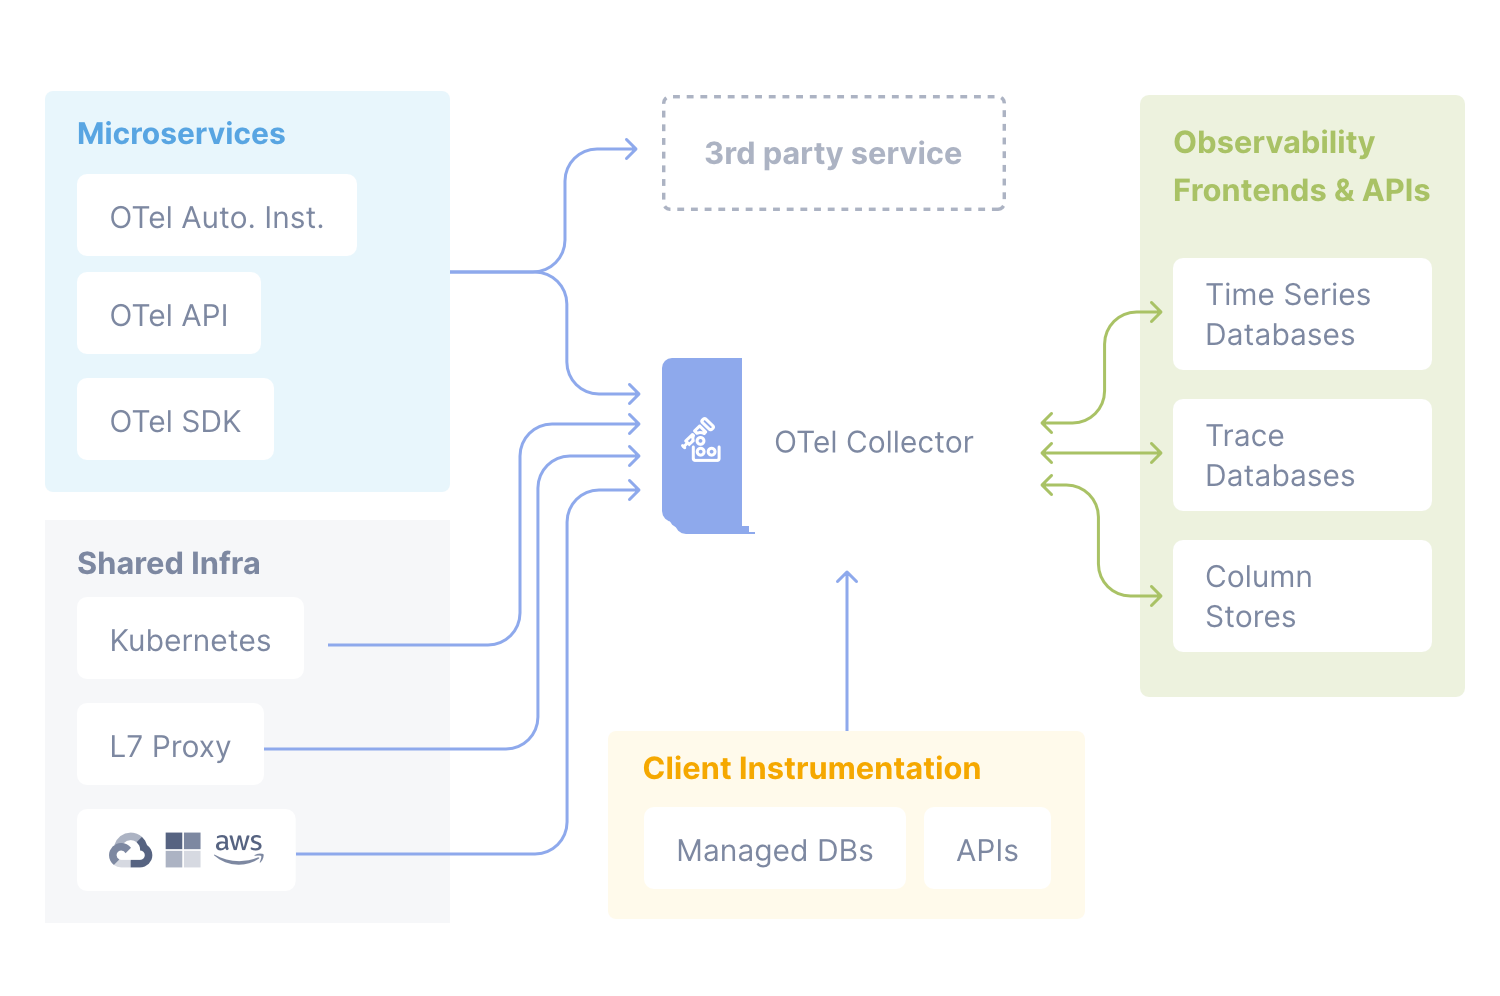
\includegraphics[width=12cm]{otel-diagram.png}
\centering
\caption{OpenTelemetry Reference Architecture.}
\label{fig:opentel-overview}
\end{figure}

Whilst tracing using a framework such as OpenTelemetry would be helpful in a larger production environment (Figure \ref{fig:opentel-overview} shows the architecture of OpenTelemetry\footnotemark{}), Omni currently only has four microservices.
Tracing has been ignored for the initial product but could easily be retrofitted around the existing logging infrastructure.
An OpenTel Exporter would then consume these traces from many different applications and publish them to a single location, for example, \underline{\href{https://prometheus.io}{Prometheus}} \nocite{prometheus}. 
The Kubernetes cluster provides top-level metrics covering basic needs, while load balancers provide more in-depth metrics, such as requests per second.
\footnotetext{`OpenTelemetry Reference Architecture' by OpenTelemetry Authors, from \url{https://opentelemetry.io/docs/}, licensed under \href{https://creativecommons.org/licenses/by/4.0/}{CC BY 4.0}.}

\section{Database}
\label{sec:impl-database}
Data is at the centre of every social media platform. The first step in creating Omni should be to build the database in which its data will be stored.
To ensure the database is reproducible on multiple servers (for example, when creating a new database shard), database migrations must be written and applied iteratively on top of one another until the final database structure has been formed. 
There are many tools and libraries for applying database migrations to a database, but since the microservices will be written in GoLang, the GoMigrate tool is a natural fit.

\subsection{Database Tables}
Figure \ref{fig:db-erd} shows the final design of the tables. The Omni platform has two main entities that are easy to see, and a third arises during the implementation.

\begin{figure}[htbp]
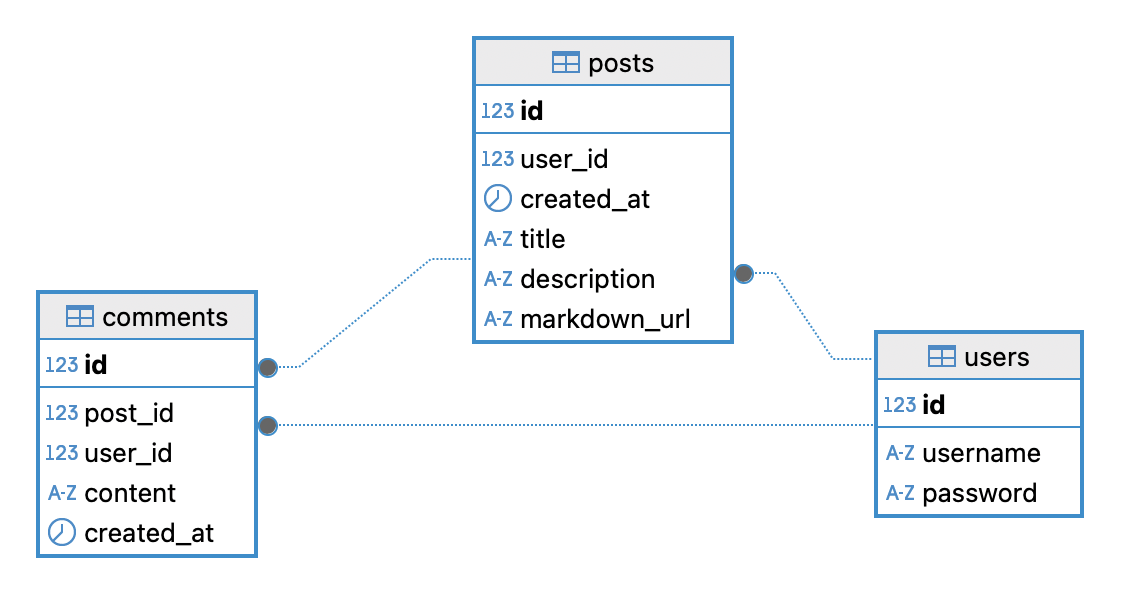
\includegraphics[width=12cm]{db-erd.png}
\centering
\caption{Database Entity Relationship Diagram}
\label{fig:db-erd}
\end{figure}

Information about each user needs to be stored, so a user table is naturally required. This includes any information about the user, such as username and password hash.
In the MVP of Omni, there is not much additional information stored about each user, but we could feasibly expand to store much more data for new features, such as storing a user's birthday.
In the future, if a hybrid approach for database distribution is used, a separate table to hold authentication data may be better to store this on a replicated database cluster rather than a sharded one.

The second easy-to-see table holds information about each post. It must store the creator's ID, title, description, link to the markdown file, timestamp, and more.
Posts will have a one-to-many relationship with users, where one user may create many posts, but each post is always associated with just one user. 

The final table is not as obvious to spot but still crucial: a table to store comments in. Storing this in the posts table does not make sense in a structured SQL database.
Adopting this approach could work in a NoSQL setup, but for popular posts, the document size would grow too big and slow down reading the post for everybody.
By storing the comments in a separate table, we can use pagination in our SQL queries to limit the number of comments we return to a user simultaneously.
This limits the load on the microservices, ensuring they are not overwhelmed by a very popular post with many comments.

\subsection{Discussion on Sharding}
As discussed in Section \ref{sec:design-system-database}, the design of the database and Snowflake IDs enable easy sharding of the database, whilst maintaining fast access times by backend microservices.
A single database has been used to maintain simplicity for the initial implementation and testing of the platform. The only difference this has in the code is that the logic for selecting which database node to retrieve data from is removed (as only one node contains all data).


\section{Backend Microservices}
\label{sec:impl-backend}
This section discusses how the backend microservices were created and how they interact with the broader environment.
Some patterns have been shared across services to enable as much code reuse as possible.

\subsection{Database Access}
\label{sec:impl-backend-db}
All three backend services require some level of database access. OmniAuth and OmniRead require only read access, whereas OmniWrite will read and write data. 

All the applications (currently) interact with the same database, although, as mentioned in Section \ref{sec:design-system-database-implementation}, future improvements could include using separate databases for things like authentication.
Because the database is shared, we can utilise the same database layer in each application, reducing the amount of code we need to write.

\subsubsection{The SQLc Library}
\underline{\href{https://sqlc.dev}{SQLc}} \nocite{sqlc} has been used to generate the database layer automatically.
This code generation library takes as input database migrations and all the queries to be run against the database.
It then compiles these inputs into type-safe code. There are multiple benefits to this approach:
\begin{itemize}
    \item Most of the code generated is boilerplate developers must write by hand or copy from documentation. It does not solve novel problems.
    \item The code generated is type-safe and handles embedding objects from joins for a more traditional object-orientated programming style. 
    \item The compiler flags breaking changes to the database via migrations when the database layer has been regenerated, but the business logic has not yet been modified.
\end{itemize}
Using this approach, SQLc has generated objects for users, posts, and comments, as well as other objects used when retrieving smaller data sections from each table.
Helpfully, the library generates an interface used within the code to access the database and an implementation of the interface for accessing the database.
However, this interface enables developers to write custom implementations, for example, to be used during unit testing. 

\lstinputlisting[language=Go, caption=The Generated GoLang Post Struct]{code-snippets/sqlc-go-models.go.bak}

All the backend services share this database layer as there is no need to write the queries separately for each one, as operations like retrieving a user profile happen in all the services.

\subsubsection{Managing Database URLs}
In order for the services to make calls to the database, they need to know where to send requests.
This is defined by a URL that is passed to each application through the environment, allowing for on-the-fly changes to the configuration without having to rebuild each application. 
The start-up function parses this URL and then creates a database connection using Go's built-in \underline{\href{https://pkg.go.dev/database/sql}{database/SQL}} \nocite{gosqlpkg} package.
Finally, a Querier object (generated by SQLc) is initialised from the database connection object. This is the object which will be passed to each service's business logic so that database requests can be made.

\subsection{Authentication}
Authentication is an important part of any platform. It ensures that users can only access data and perform tasks they are authorised to do. 
Rather than using an authentication library, Omni uses a simple, custom authentication implementation, where users log in using a username and password.

\subsubsection{Sign Up}
\label{sec:impl-auth-signup}
When a user signs up to Omni, they enter a unique username and a password of their choice.
This information is sent to the backend, where the password is hashed using the bcrypt algorithm developed by \citeauthor{provos1999future}.
The GoLang package \underline{\href{https://pkg.go.dev/golang.org/x/crypto/bcrypt}{crypto/bcrypt}} \nocite{gobcryptpkg} handles this. The password hash is then stored in the database along with the rest of the user's details.

\subsubsection{Bcrypt}
The Bcrypt algorithm stores all the information required to verify a password attempt in the hash.

\begin{figure}[htbp]
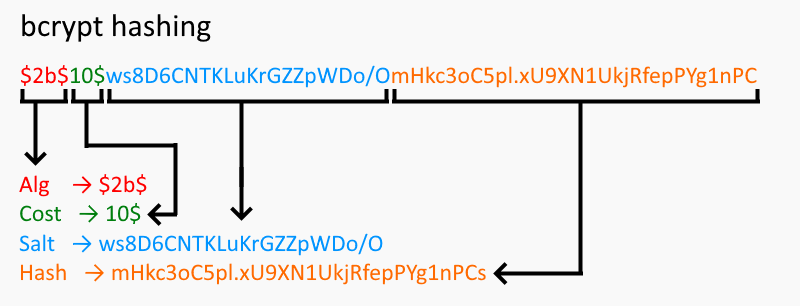
\includegraphics[width=12cm]{bcrypt-parts.png}
\centering
\caption{Sections of the Bcrypt Hash}
\end{figure}

The first section of the hash contains the algorithm used to create it. Bcrypt uses a version of the Blowfish cypher, denoted by the hash \verb|$2b$|.
The second section is the cost factor used in the algorithm. The default of 10 is used for Omni, but in production, this should be increased to 12 or higher.
Generally, the larger the value of the cost factor, the slower it is to check a password.
While counter-intuitive, this is the desired behaviour, as the slower it is to check a password, the harder it is for a brute-force algorithm to check the most common passwords.
The third section of the hash is the salt used; this is stored as plain text so that it can be used to derive the encryption key for later use.
Finally, the encrypted password is stored as the last part of the hash, which is compared against a potential password.

Checking a password involves deriving the encryption key from the given algorithm, cost factor and salt, using that key to encrypt the given password and then comparing it against the valid password hash. If the hashes match, the password is valid.

\subsubsection{JSON Web Tokens}
JWTs are the industry standard for ongoing authentication. They can contain many standard or custom `claims', which the application uses to determine whether the JWT is valid.
In particular, Omni uses the \verb|exp| and \verb|sub| claims (standing for expires at and subject, respectively). 

After a JWT body is generated, applications hash it using a secret key, which is appended to the JWT to ensure that the body is not modified by anyone other than the authorised applications. 
Figure \ref{fig:jwt-parts} shows the three sections of a JWT.

\begin{figure}[htbp]
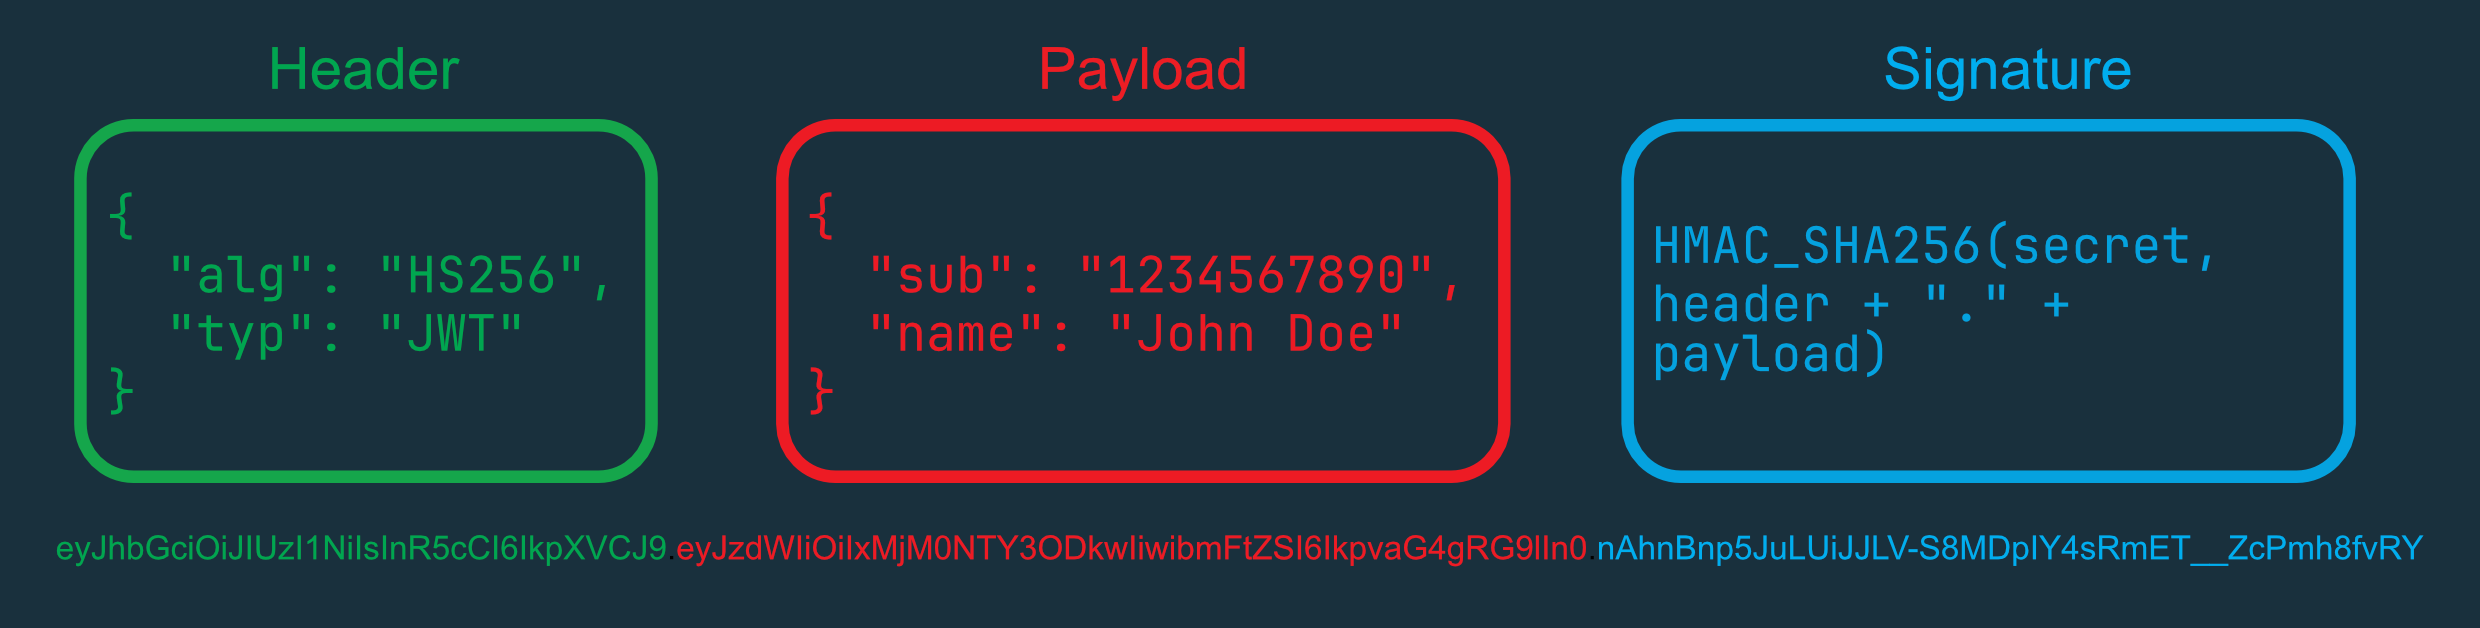
\includegraphics[width=12cm]{jwt-parts.png}
\centering
\caption{Sections of a JSON Web Token}
\label{fig:jwt-parts}
\end{figure}

In subsequent requests to restricted endpoints, clients attach their JWT in the Authorization header of the HTTP request.
The relevant backend, which handles requests to that particular endpoint, can then verify the claims in the JWT.
Based on the subject claim of the JWT, the backend can decide if the client making the request is authorised to do so for the particular action they are performing.
For example, a user can delete a post they have created but cannot delete posts from other users.

\subsection{Middleware}
Middleware is software that sits between the client request and the final logic that handles that request.
It can achieve various effects, from modifying the request to rejecting it altogether (due to a lack of authentication, for example). 

Middleware is crucial in modern web services, even more so in a microservices architecture.
Omni utilises middleware for safety, stability, and functionality. 

The most crucial and ubiquitous of Omni's middleware is the logging middleware.
This middleware records each incoming request as a log, and after the request is processed, it logs the amount of time taken to serve that request. 
These logs follow a structured format, allowing external monitoring tools to use them to build a better understanding of how long requests take to process on average and which types of requests take the longest.
This allows bottlenecks to be identified. Appendix \ref{sec:apdx-middleware-implementations} shows the implementation of this simple yet powerful middleware.

Another important middleware that Omni takes advantage of is MaxBytesReader.
This middleware sets the maximum number of bytes that can be read from the body of an HTTP request to be 1 MiB.
The middleware prevents DDOS attacks using vast HTTP request bodies, where the application may run out of memory trying to decode all the information in the body.
For all the Omni endpoints, the expected amount of data should never exceed 1 MiB, so any request with a body larger than that should be rejected with an error.

\subsection{OmniAuth}
The simplest of the backend services is OmniAuth, which authenticates an existing user to access restricted endpoints.
OmniAuth serves just one endpoint: \verb|POST /api/login|. The handler expects the request to have a JSON body with the fields \verb|username| and \verb|password|. 
The username is used to retrieve the user from the database. When the user does not exist, the endpoint returns a 404 Not Found HTTP error.
The returned data from the database includes the Bcrypt hash of the user's password. 

As mentioned above in Section \ref{sec:impl-auth-signup}, the \underline{\href{https://pkg.go.dev/golang.org/x/crypto/bcrypt}{crypto/bcrypt}} \nocite{gobcryptpkg} package compares the password sent in the request to the hashed password stored in the database.
If the passwords match, the authentication request is valid. If they do not match, the request returns a 401 Unauthorised HTTP error.

Given that the passwords match, OmniAuth will create a JSON Web Token (JWT) (code shown in Listing \ref{lst:go-jwt}) that can be used to authenticate the user for subsequent requests to restricted endpoints.

\lstinputlisting[language=Go, caption=Example of Creating a JWT, label={lst:go-jwt}]{code-snippets/go-jwt-creation.go.bak}

\subsection{OmniRead}
OmniRead, as described in Section \ref{sec:design-system-backend}, is responsible for handling any HTTP Get requests. This allows us to scale read requests separately from the scaling of backend services that handle write requests.
In the initial version of Omni, the data that users need to be able to read is: 
\begin{itemize}
    \item Posts
    \item Users
    \item Comments
\end{itemize}
However, we have more than three endpoints, as users may want to access different data sections differently. For example, a user may want to retrieve all the posts a user has created and the most recent posts by any user. 

All the API endpoints served by OmniRead are unauthorised, meaning that anybody can access them without a JWT token. This simplifies the service regarding the middleware required for each endpoint and its runtime configuration in the Kubernetes environment. 

For some endpoints that could return infinite amounts of data, such as retrieving comments on a post or posts by a particular user, paging is needed.
This ensures that the database and the backend service are not overwhelmed by a denial-of-service attack, where a malicious request can cause the entire service to hang or run out of memory while processing it. 
Paging ensures that the data returned has a maximum size of ten items. Users who wish to see more items can request the next page, which will return the following ten items.

Achieving this paging in the application layer is trivial, but it still leaves the attack vector open. In this scenario, the application layer would still require all the data from the database, even if it only returned a subset to the user. 
Luckily, popular SQL databases already have this paging feature built-in through the \verb|LIMIT| and \verb|OFFSET| keywords.
\verb|LIMIT|, as the name suggests, limits the number of rows of data returned, and \verb|OFFSET| skips the number of rows specified.
For example, with a \verb|LIMIT| of 10 and \verb|OFFSET| of 0, the first 10 rows will be returned. With an \verb|OFFSET| of 10, rows 11-20 are returned. 

\lstinputlisting[language=SQL, caption=Example of SQLc Query with LIMIT and OFFSET]{code-snippets/sql-limit-example.sql}

Other paging strategies also exist. For example, in the context of comments, a user may prefer to page by time, finding all the comments before or after a timestamp.
This paging application is more useful for other applications that use the API, perhaps for research purposes.
In contrast, users interacting with the Omni platform via the website will likely want to read the most recent comments on a post or the highest-rated comments if a liking system is introduced.
The \verb|LIMIT| and \verb|OFFSET| approach is more efficient for these cases when compared to the client specifying a timestamp or other parameter to find comments before or after, with different sorts applied to the query. 

OmniRead returns data in the response body in a JSON format. JSON is the standard format for transmitting data in APIs on the web.
Whilst other more efficient formats exist, such as \underline{\href{https://protobuf.dev}{ProtoBuf}} \nocite{protobuf}, JSON is ubiquitous and well-supported by most languages' standard libraries.
GoLang has powerful, built-in tooling to encode and decode to and from the JSON format into standard GoLang structs.
As part of a set of helper functions for all the backend services, Omni has a helper function that takes an object and an HTTP Response Writer object and writes the JSON encoding of the object to the response along with a 200 Success HTTP code.
This helper function is used across all the backend services to transmit data to the request sender. 

\lstinputlisting[language=Go, caption=Example of Writing JSON to the Response, label={lst:go-json}]{code-snippets/encode-json-helper.go.bak}

\subsubsection{Conforming to the HTTP Specification}
Throughout the OmniRead service (and all the backend services), Omni attempts to conform as much as possible to the uniform HTTP interface defined by \citeauthor{fielding1999rfc2616}.
In practice, this means reflecting as much information as possible through HTTP Status Codes and adopting the correct HTTP verbs.
Some examples include 200 Success and 201 No Content when requests are successful, with the former indicating there is some returned content in the body of the response, whilst the latter means nothing was returned.
When a request is malformed or otherwise incorrect, status codes in the range 4XX are returned depending on the type of error.
Finally, the service returns 500 Internal Server Error and 503 Service Unavailable errors when the backend encounters errors it cannot recover from, such as the database being down. 

Consumers of the API should be able to use HTTP Status Codes as the first port of call to immediately know if a request was successful, rather than the way that some more modern JavaScript frameworks hide errors inside of 200 Success messages.
The practice of hiding errors inside responses that return with a 200 code can lead to poor error handling and unexpected fatal crashes.

As discussed by \citeauthor{richardson2008restful}, ``when the method information isn’t found in the HTTP method, the interface stops being uniform.''
It is important to conform as much as possible to the specifications that underpin the modern web; otherwise, the tooling and developers working on the web will have to work harder to achieve the same baseline of safety.

\subsection{OmniWrite}
OmniWrite handles requests that could modify the database, such as creating a post or adding a new user. 
For each class of resource, user, post, and comment, OmniWrite handles three endpoints:
\begin{itemize}
    \item POST - Creates a new object
    \item PUT - Updates an existing object by its ID
    \item DELETE - Deletes an existing object by its ID
\end{itemize}
The implementation for each class is mostly the same, with the only difference being the data associated with each resource in the class.
For example, the implementation of creating a new comment or post is almost the same, except for the data expected in the request body and the database calls made. 

The general skeleton for the implementation of each handler for this service follows the following blueprint:
\begin{enumerate}
    \item For PUT and DELETE requests, parse the ID parameter from the request's path and check if the resource exists in the database.
    \item For POST and PUT requests, decode the request's body to find the new parameters.
    \item Call the relevant function in the database layer.
    \item Check for errors and return the response to the client.
\end{enumerate}
Before modifying the database, the handler must also verify that the caller provided a valid JWT for the request.
The only exception is when creating a new user (as the user will not yet have created their password or possess a JWT). 

A JWT is valid for a PUT or DELETE request if the resource owner matches the user ID in the subject field and the token has not expired.
The only other thing that complicates the request handlers in OmniWrite is the amount of places where errors can arise. 
The error handling logic is responsible for over half of the code in each handler, ensuring that each response receives the correct HTTP status code, depending on the type of error.

\subsection{OmniView}
OmniView is the application responsible for serving HTML to browsers when a user navigates to the Omni website.
Whereas the other three services all serve JSON content in their responses, OmniView responds with HTML, CSS, and JS, which the browser can use to render content on screen for a user.
There are many different methods, tools, and frameworks for building a website, such as ReactJS, NextJS, Java Spring Boot, and plain HTML \citep{StackOverflow2024}

Writing static HTML pages which are served to browsers is not very common in the industry now, with contemporary solutions (even those with static sites with no dynamic content) use frameworks to generate the HTML from an easier language to work with. 

Given that the web pages OmniView will be serving have dynamic designs but limited complex user interaction, HTMX and TailwindCSS will be used to render the HTML content that will be sent to browsers.
HTMX is a lightweight JavaScript library that enables dynamic web interactions through HTML attributes.
It allows parts of a page to be updated dynamically in response to events without writing any custom JavaScript. It keeps the rendering of HTML on the server side while maintaining the state through the URL of a webpage. 

Some modern JavaScript frameworks prefer to use a single-page application, where the URL does not change when navigating to entirely new pages, instead powering all interaction through client-side rendering.
However, this can lead to much more complex JavaScript running on the client than is necessary, increasing the amount of data that needs to be sent when the page is loaded.
By keeping this processing on the server, OmniView only needs to send each client the rendered page for them to view, lowering the network cost of each request. 

TailwindCSS on the other hand, is a CSS framework that provides low-level utility classes to build custom, responsive designs quickly.
Rather than writing custom classes for each component, Tailwind allows for the composition of utilities directly on HTML elements, increasing the locality of code and enabling rapid development and consistent styling. 

\lstinputlisting[language=HTML, caption=Example of TailwindCSS Classes]{code-snippets/tailwind-example.html}

The combination of GoLang, HTMX, and TailwindCSS will enable Omni to serve fast, beautiful, and responsive web pages even with limited bandwidth. 

The first step in creating OmniView is to set up the web server and ensure that it is serving static content.
The CSS file each page will reference is the static content to be served in the case of OmniView.
The Tailwind command line tool generates this content by scanning all the project's HTML files, extracting the Tailwind classes used, and compiling the styling for each one into a minified CSS file.
Generating the CSS file this way ensures that only the Tailwind styles the website uses are sent to the client, keeping response sizes low.

The second step is to produce the website's HTML.
The HTML is produced using GoLangs built-in templating language, enabling the reuse of standard sections like the navigation bar or footer and dynamic insertion of variables from the application, such as post titles.
The templates also include HTMX in the elements to enable dynamic content updates, for example, when a new comment is added.
Rather than reloading the whole page when a user adds a comment, we can dynamically insert the new comment at the top of the list so that the user can see the result of their interaction straight away, with a minimal impact on the network.

While the frontend design is not the primary focus of this project, efforts were made to create a responsive, accessible design which is easy for users to navigate.
Some screenshots can be found in Appendix \ref{sec:apdx-screenshots}.

\subsection{Serving Content}
With these basic components in place, the next stage of development is to start creating the handlers for each application endpoint.
Most pages require a database call to retrieve the content that will be displayed. This is handled by making a request to the relevant backend service so as not to duplicate work already done. 

In cases where multiple pieces of data are needed, such as viewing a user's page (which requires a call to load the information about the user and a separate call to load all the posts by that user), OmniView leverages GoLangs' concurrency features.
These features enable both requests to be made concurrently with full cancellation support.
Appendix \ref{sec:apdx-concurrency-omni-view} contains a shortened example of this code.

Once all the required requests have been completed, the code stops waiting and the response data object is formed.
The template renderer receives this data object as input so that it can replace any fields in the template with the relevant data, before sending the rendered HTML in the response of the HTTP request.

\subsection{Authentication in OmniView}
Authentication needs to be handled slightly differently in OmniView compared to OmniWrite.
This need is because the browser does not have a way to automatically set the Authorisation header when it makes requests to the web server.
Instead, authentication data is transmitted and stored in a cookie. The browser knows to send cookies related to a website with every request it makes. 

When a user signs into Omni via the website, the same JWT is produced by the backend.
However, before the response is sent to the user via OmniView, the JWT is set as the value of a cookie, which is also sent back to the browser.
When the browser receives this response, it saves the cookie to its local storage and transmits it along with every subsequent request it makes before the cookie's expiry timestamp. 

\begin{figure}[htbp]
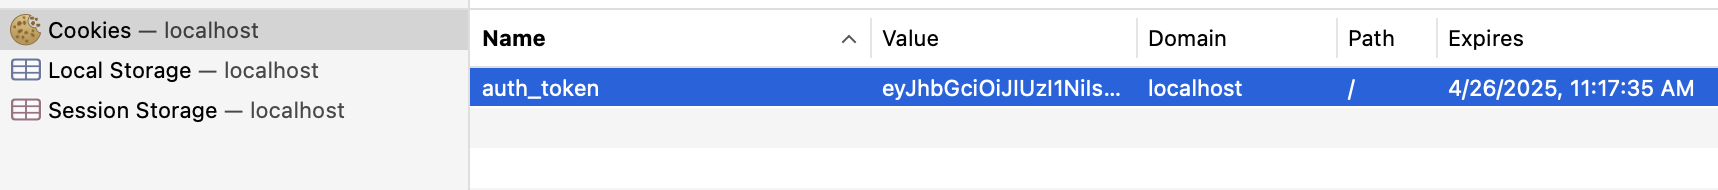
\includegraphics[width=12cm]{cookie.png}
\centering
\caption{Authentication Cookie Set by OmniView}
\label{fig:auth-cookie}
\end{figure}

When OmniView receives a request, middleware checks if the cookie is present and that the JWT inside the cookie is valid for the request.
If both of these checks are true, the request is processed as it would be normally, and the response is sent.
If the cookie is not present or is not valid, OmniView sends a redirection status code and redirects the browser to the login page, where the user can enter their credentials to receive a new cookie.

\section{Load Balancer}
Many backend services are required to handle the load for a platform to scale efficiently.
Requests should be distributed evenly across each service for a platform to work optimally. A load balancer is required to achieve optimal performance.
Omni has a custom, configurable load balancer that serves different paths to different backends.

\subsection{Note on Load Balancing in the Final Version of Omni}
The original plan was to use a custom load balancer for the Omni platform to prevent vendor lock-in to a particular cloud service's load balancer.
However, after carefully reviewing the Kubernetes documentation, particularly the relatively new Gateway API, the decision was made not to deploy the custom load balancer but rather to use the Gateway API to provision a load balancer from the cluster provider.
This decision allows Omni to remain cloud-portable, allowing the Gateway API to automatically provision a cloud provider's load balancer. 

Some work was needed to enable a load balancer in a custom-built, bare-metal Kubernetes cluster such as the one Omni was tested on (2x Raspberry Pis); however, \underline{\href{https://metallb.io}{MetalLB}} \nocite{metallb} and \underline{\href{https://docs.nginx.com/nginx-gateway-fabric/}{NGINX Gateway Fabric}} \nocite{nginxgatewayfabric} were successfully implemented and used for testing.

\subsection{Configuration}
The Omni load balancer begins with the configuration. The configuration defines which load balancing algorithm to use (for example, the round-robin algorithm) and which paths the load balancer should expose. 

The load balancer ingests this configuration file (written in YAML), on start-up and creates internal maps for each path.
It also exposes the standard liveness endpoints \verb|/livez| and \verb|readyz|. \verb|readyz| responds with a healthy status code when a backend exists and is ready to serve responses for each path defined in the configuration.

\subsection{The Load-Balancing Pool}
Two other endpoints are also exposed: \verb|addz| and \verb|removez|. The backends use these endpoints to register and unregister themselves from the load-balancing pool. 
When a backend adds itself to the load-balancing pool, a reverse proxy is created for the backend's IP address and added to the pool.
When a client sends a request via the load balancer, the new backend will be available for the selected algorithm to choose from.

\begin{figure}[htbp]
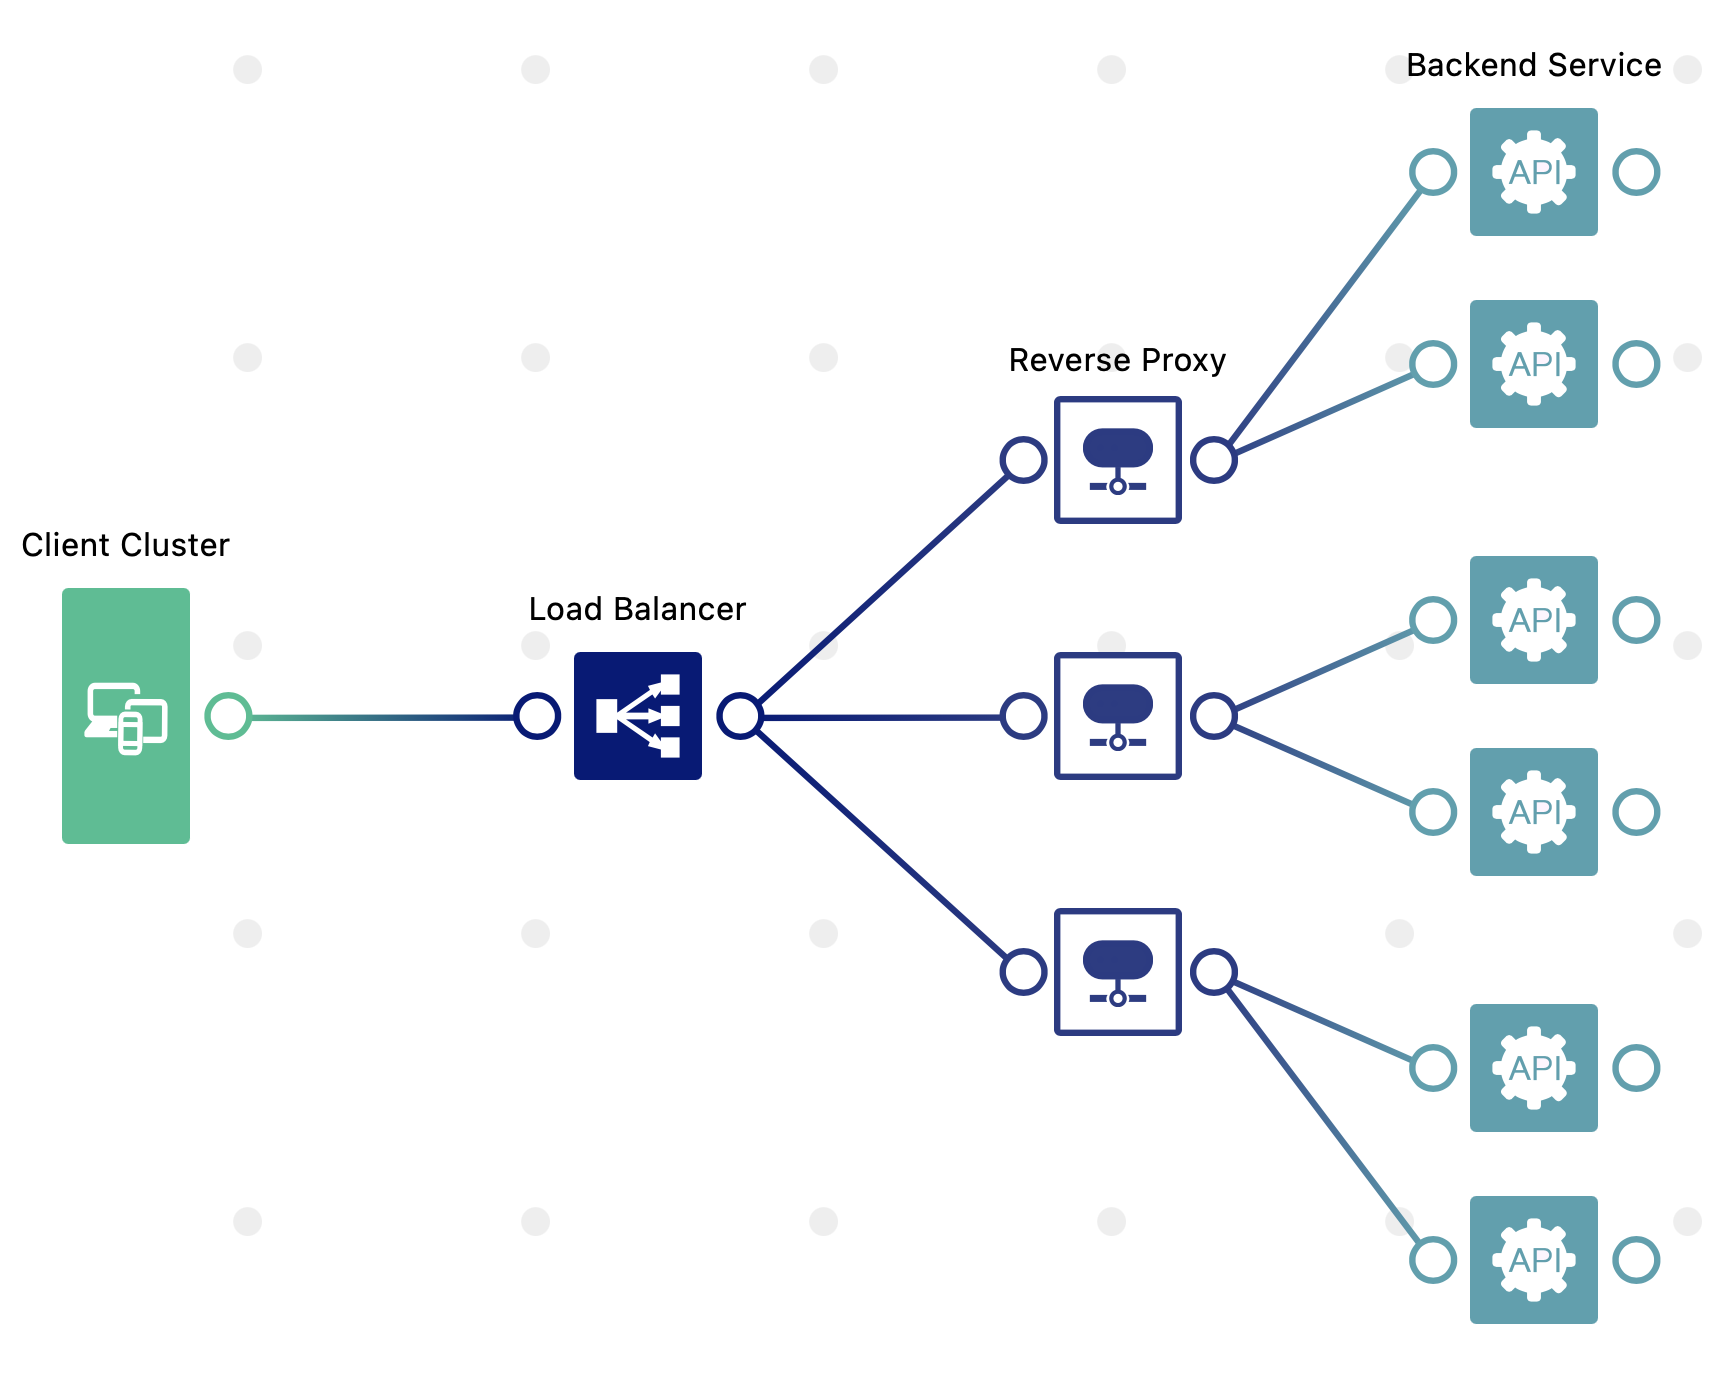
\includegraphics[width=12cm]{loadbalancer-design.png}
\centering
\caption{Load Balancer Design Overview}
\label{fig:loadbalancer-design}
\end{figure}

Once the chosen algorithm has picked a backend to serve the user's request, the load balancer forwards the request to the backend using its direct IP address.
The request is also modified to include the \verb|X-Real-IP| and \verb|X-Proxy| headers to indicate to the backend nodes that the load balancer has forwarded this request and from whom the request originated. 

The load balancer is also responsible for regularly checking that the registered backends are still alive and healthy. When a backend does not respond before the timeout, it is removed from the healthy pool of nodes until it responds again or is removed from the load-balancing pool altogether.

\begin{figure}[htbp]
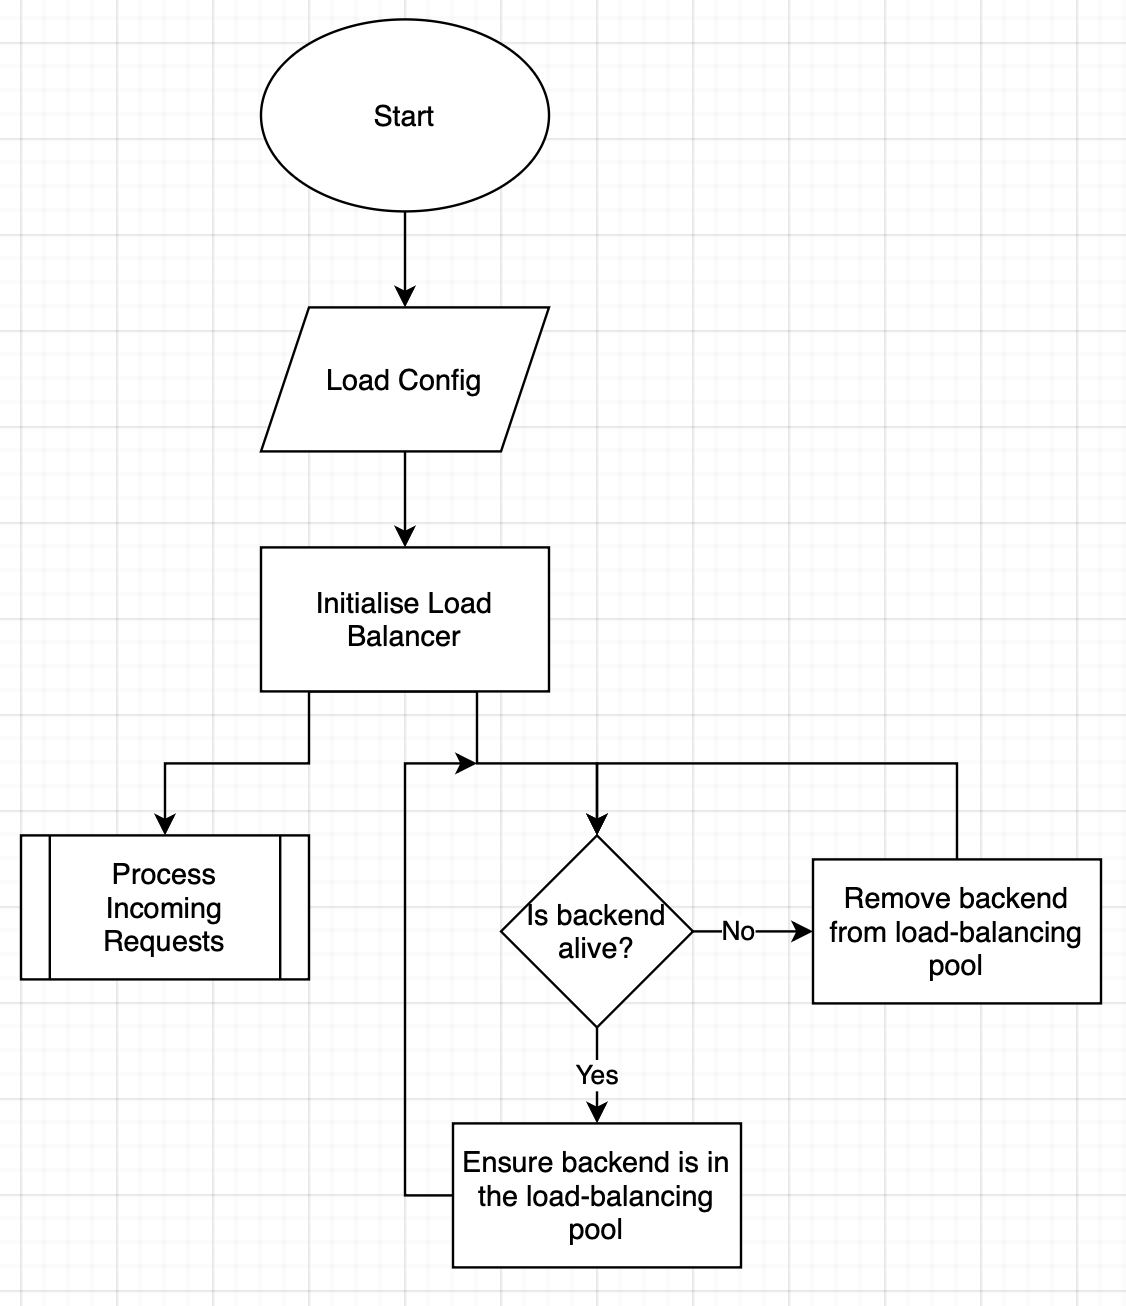
\includegraphics[width=12cm]{load-balancer-flow.png}
\centering
\caption{Load Balancer Flow}
\label{fig:loadbalancer-flow}
\end{figure}

\subsection{Load-Balancing Algorithms}
Many different load-balancing algorithms exist, and this report does not discuss the benefits and drawbacks of each.
For the first implementation of the load balancer, a simple round-robin algorithm was implemented; however, much more complex and efficient approaches are available, such as the least connections and least response time algorithms.
The study by \citeauthor{sharma2008performance} into the performance of different load-balancing algorithms is particularly informative.

\section{Kubernetes and Deployment}
Now that each platform component is built, it needs to be deployed to work in unison. As mentioned in Section \ref{sec:design-system-kubernetes}, the microservices will be deployed into a Kubernetes cluster to enable easy inter-pod communication, autoscaling, deployment rollouts with zero downtime, and more.
The database will not be deployed into Kubernetes as this does not follow the industry standard practices surrounding data storage. 

Kubernetes pods are ephemeral, meaning they should be stateless themselves and able to be killed and restarted without interrupting the application they serve. 
This design contradicts the stateful design of databases (otherwise, they would not be helpful) that should be resilient to failure. 

\subsection{Kubernetes Manifests}
Whilst Kubernetes clusters can be configured and interacted with via a command-line tool, the industry leans towards using Infrastructure-as-Code (IAC for short), which allows infrastructure to be version-controlled using Git like the applications it hosts.
IAC brings a whole host of benefits other than version control, such as the ability to tear down and rebuild environments quickly and easily through virtualisation \citep{huttermann2012infrastructure}.

Two main parts are needed to deploy the services to Kubernetes: a deployment and a service. The \underline{\href{https://kubernetes.io/docs/home/}{Kubernetes Official Documentation}} \nocite{kubernetesdocs} describes each best:
\begin{itemize}
    \item ``A Deployment manages a set of Pods to run an application workload, usually one that doesn't maintain state.''
    \item A service allows one to ``expose an application running in your cluster behind a single outward-facing endpoint, even when the workload is split across multiple backends.''
\end{itemize}

In layman's terms, a deployment manages a set of pods, ensuring that if one dies, another takes its place, whilst a service allows the outside (or inside) world to communicate with said pods through a single interface.
Services are the key to communication between different backends inside of a cluster.
Rather than a backend needing to find the IP of a specific pod to serve its request, it can send the request to the service, which, in turn, will forward it to the pods it manages. 

A deployment and service manifest has been created to manage the underlying pods for each Omni service: OmniRead, OmniWrite, OmniView, and OmniAuth.
The deployment manifest also includes the environment variables that power each service's configuration, including the database connection URL and the port via which to connect.

\subsubsection{A Word on Helm}
Helm is an open-source package manager which simplifies the management of Kubernetes deployments. It allows for the installation of predefined standalone units into a cluster. 
The configuration of Omni's deployment into Kubernetes has been written as a Helm chart, allowing for easy deployment and upgrade during its development lifecycle. 
Charts are written using the GoLang templating language, allowing the same chart to be reused across multiple environments (say, a test cluster versus a production cluster).
Variables defined in the chart are replaced with different values.

\subsubsection{Cluster Ingress}
By default, services use the ClusterIP type, which exposes the service internally to other members of the cluster.
While this may be perfect for some applications, Omni needs some sort of connection to the outside world to be functional.
Traditionally, a Kubernetes Ingress would be used; however, the new Gateway API allows for a more portable definition. 

Alongside the Deployment and Service for each backend application, Omni's Chart includes Gateway and HTTPRoute manifests.
The documentation defines the Gateway as ``an instance of traffic handling infrastructure, such as cloud load balancer.''
In the case of the bare-metal cluster Omni has been tested on, under the hood, this will link through the NGINX Gateway Fabric to the MetalLB load balancer, providing an external IP address to the Gateway. 
The second part of the puzzle is the HTTPRoute. Again, the documentation defines this as ``HTTP-specific rules for mapping traffic from a Gateway listener to a representation of backend network endpoints. These endpoints are often represented as a Service.''
The HTTPRoutes specify the destination for an incoming request. 
For instance, GET requests to a path beginning \verb|/api/| should be sent to the OmniRead service. 

\begin{figure}[htbp]
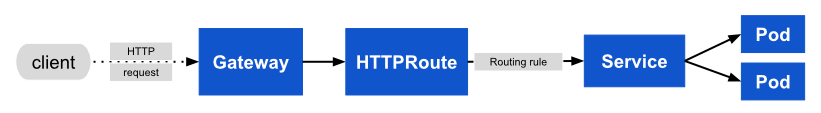
\includegraphics[width=12cm]{gateway-request-flow.png}
\centering
\caption{Flow of a Request through the Gateway}
\label{fig:k8s-gateway-flow}
\end{figure}

Combining the HTTPRoute and Gateway allows Omni to communicate via a single external IP while sharing requests across many backend applications to balance the load and service the requests.
Figure \ref{fig:k8s-gateway-flow} \footnote{`Kubernetes Gateway Flow' by The Kubernetes Authors, from \url{https://kubernetes.io/docs/concepts/services-networking/gateway/}, licensed under \href{https://creativecommons.org/licenses/by/4.0/}{CC BY 4.0}.} shows the flow of a request through the Gateway and HTTPRoutes.

\subsubsection{Automatic Horizontal Scaling}
The final piece of the Kubernetes puzzle is configuring the deployments to automatically scale horizontally (create new pods) as load increases.
The key to this is using a \underline{\href{https://kubernetes.io/docs/tasks/run-application/horizontal-pod-autoscale/}{HorizontalPodAutoScaler}} \nocite{horizontalpodautoscaler} manifest, which defines the rules for how deployments should scale their pods.
In the case of Omni, using CPU utilisation is the simplest solution. However, more complicated metrics, such as requests per second, could be used.
The auto-scaler targets a CPU utilisation of 50\% for each pod. The deployment specifies the minimum amount of CPU and memory that a pod requires to run and the maximum a pod can use.
The utilisation of each pod is calculated based on the limits specified.
As utilisation increases over 50\%, the auto-scaler triggers the creation of more pods.
Once the period of high load ends, the auto-scaler waits for a specified period before scaling the pods down to their nominal amount again.

\begin{figure}[htbp]
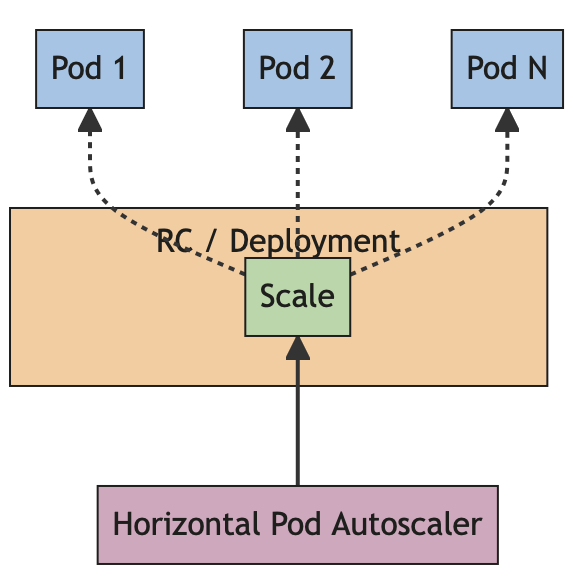
\includegraphics[width=12cm]{horizontalpodscaling.png}
\centering
\caption{HorizontalPodAutoscaler controls the scale of a Deployment and its ReplicaSet}
\label{fig:horizontalpodscaling}
\end{figure}

Figure \ref{fig:horizontalpodscaling} \footnote{`HorizontalPodAutoscaler' by The Kubernetes Authors, from \url{https://kubernetes.io/docs/tasks/run-application/horizontal-pod-autoscale/}, licensed under \href{https://creativecommons.org/licenses/by/4.0/}{CC BY 4.0}.} demonstrates how the HorizontalPodAutoscaler works with the Deployment and ReplicaSet to scale the number of pods up and down as required.
